\documentclass[11pt]{article}

%==================== Packages ====================
\usepackage[utf8]{inputenc}
\usepackage[T1]{fontenc}
\usepackage[margin=1in]{geometry}
\usepackage{amsmath,amssymb,amsthm}
\usepackage{mathtools}
\usepackage{tikz}
\usetikzlibrary{arrows.meta, positioning, shapes.geometric, calc}
\usepackage{algorithm}
\usepackage{algpseudocode}
\usepackage{float}
\usepackage{enumitem}
\usepackage{hyperref}
\hypersetup{colorlinks=true,linkcolor=blue,citecolor=blue,urlcolor=blue}

%==================== Theorem environments ====================
\newtheorem{theorem}{Theorem}
\newtheorem{lemma}{Lemma}
\newtheorem{corollary}{Corollary}
\theoremstyle{definition}
\newtheorem{definition}{Definition}
\newtheorem{problem}{Problem}
\theoremstyle{remark}
\newtheorem{remark}{Remark}

%==================== Macros ====================
\newcommand{\OPT}{\mathrm{OPT}}
\newcommand{\OPTfrac}{\OPT_{\mathrm{frac}}}
\newcommand{\OPTSF}{\OPT_{\mathrm{SF}}}
\newcommand{\ALG}{\mathrm{ALG}}
\newcommand{\ALGSP}{\ALG_{\mathrm{SP}}}
\newcommand{\ALGSF}{\ALG_{\mathrm{SF}}}
\newcommand{\ESF}{E_{\mathrm{SF}}}
\newcommand{\GSF}{G_{\mathrm{SF}}}
\newcommand{\VSF}{V_{\mathrm{SF}}}
\newcommand{\src}{\mathrm{src}}
\newcommand{\dst}{\mathrm{dst}}
\newcommand{\dem}{\mathrm{dem}}
\newcommand{\len}{\mathrm{len}}
\newcommand{\Tin}{T^{(i)}_{\mathrm{in}}}
\newcommand{\Tout}{T^{(i)}_{\mathrm{out}}}
\newcommand{\din}{d_{\mathrm{in}}}
\newcommand{\dout}{d_{\mathrm{out}}}
\newcommand{\Din}{D^{(i)}_{\mathrm{in}}}
\newcommand{\Dout}{D^{(i)}_{\mathrm{out}}}
\newcommand{\Zzero}{\mathbb{Z}_{\ge 0}}
\DeclareMathOperator{\SP}{SP}

\title{\bf Minimum Aged Labelling with Capacity Constraints:\\[2pt]
A $\theta$-Threshold Two-Track Flow-Splitting Algorithm}
\author{}
\date{}

\begin{document}
\maketitle

\begin{abstract}
We study \emph{Minimum Aged Labelling with Capacity constraints} (MAL-C), a temporal
network-design problem: on an edge-weighted directed graph we must assign every edge a set of
departure times and route a set of demands, so as to minimize the total number of unit-capacity
vehicle dispatches. We give a polynomial-time approximation algorithm. It splits each demand into an
integer part, routed along shortest paths, and a fractional part, consolidated onto a shared Directed
Steiner Forest backbone; a threshold $\theta$ balances the two tracks. Choosing $\theta$ optimally
yields an $O\!\left(\sqrt{h}\,n^{1/3}+n^{2/3}\right)$-approximation, where $n$ is the number of
vertices and $h$ the number of demands.
\end{abstract}

%====================================================================
\section{Preliminaries and Problem Statement}\label{sec:prelim}
%====================================================================

In a \emph{temporal} (time-varying) network, an edge may be traversed only at certain prescribed
times. This section fixes the temporal-graph vocabulary, recalls the Minimum Aged Labelling problem,
and states the capacity-constrained variant we study.

\subsection{Temporal graphs and temporal paths}\label{sec:temporal}

We work throughout with an edge-weighted directed graph $G=(V,E)$ and a \emph{travel-time} function
$w:E\to\mathbb{N}$; flow that enters an edge $e$ at time $t$ arrives at the head of $e$ at time
$t+w(e)$. We write $n=|V|$ and $m=|E|$.

\begin{definition}[Temporal graph]\label{def:tgraph}
A \emph{temporal graph} $(G,\lambda)$ is the graph $G=(V,E)$ together with a \emph{label function}
$\lambda:E\to 2^{\Zzero}$, where $\Zzero=\{0,1,2,\dots\}$ and $\lambda(e)$ is the set of times at which
edge $e$ may be entered (the \emph{labels} of $e$).
\end{definition}

\begin{definition}[Temporal path, temporal connectivity]\label{def:tpath}
A \emph{temporal path} from $u$ to $v$ in $(G,\lambda)$ is a sequence
$(e_1,t_1),(e_2,t_2),\dots,(e_\ell,t_\ell)$ satisfying:
\begin{itemize}[topsep=2pt,itemsep=2pt]
  \item \emph{Path connectivity:} each $e_i\in E$, and $e_1e_2\cdots e_\ell$ is a walk from $u$ to $v$
        in $G$;
  \item \emph{Time monotonicity:} $t_i\in\lambda(e_i)$ for every $i$, and, writing $e_i=(v_i,v_{i+1})$,
        \[
          t_{i+1}\;\ge\;t_i+w(e_i)\qquad(1\le i<\ell).
        \]
\end{itemize}
The monotonicity condition encodes travel time: departing $v_i$ at $t_i$, the flow reaches $v_{i+1}$
at time $t_i+w(e_i)$, so the next departure $t_{i+1}$ cannot precede that arrival (in the classical
unit-time case $w\equiv 1$ it becomes the strict increase $t_1<t_2<\dots<t_\ell$). We say $(G,\lambda)$
is \emph{temporally connected} on a set of ordered vertex pairs if each such pair admits a temporal
path.
\end{definition}

\subsection{The Minimum Aged Labelling problem}\label{sec:mal}

Minimum Aged Labelling (MAL), introduced by Carnevale et al.~\cite{CDO25}, asks for a labelling that
uses as few labels as possible while making the graph temporally connected.

\begin{problem}[Minimum Aged Labelling (MAL)]\label{prob:mal}
\leavevmode
\begin{description}[topsep=2pt,itemsep=1pt,leftmargin=6.5em,style=nextline]
  \item[\textnormal{Input:}] a digraph $G=(V,E)$ and a maximum-label bound $a\in\mathbb{N}$.
  \item[\textnormal{Output:}] a label function $\lambda:E\to 2^{\mathbb{N}}$.
  \item[\textnormal{Constraints:}] $(G,\lambda)$ is temporally connected (between every ordered pair
        of vertices), and $\lambda(e)\subseteq\{1,\dots,a\}$ for every $e$.
  \item[\textnormal{Objective:}] minimize the total number of labels $\displaystyle\sum_{e\in E}|\lambda(e)|$.
\end{description}
\end{problem}

\subsection{Minimum Aged Labelling with capacity constraints}\label{sec:malc}

In practice demands are heterogeneous: the amount that must cross an edge at a given time may require
several unit-capacity vehicles. \emph{Minimum Aged Labelling with Capacity constraints} (MAL-C)
captures this by charging each edge $e$, at each departure time $t$, for the number of unit-capacity
vehicles needed to carry the flow that departs on $e$ at time $t$ (formally, the
objective~\eqref{eq:objective}).

The variant we study augments MAL with edge travel times $w$, a demand set with real-valued amounts,
and the capacity objective; and it simplifies MAL in two ways: there is \emph{no} maximum-label bound
(a label may be any time in $\Zzero$), and all demands are available from time $0$ (a common release
time). Flow is splittable, and nodes have unlimited buffering: a demand may wait at a node for any
amount of time.

\begin{problem}[MAL-C, the variant studied here]\label{prob:malc}
\leavevmode
\begin{description}[topsep=2pt,itemsep=1pt,leftmargin=6.5em,style=nextline]
  \item[\textnormal{Input:}] an edge-weighted digraph $G=(V,E)$ with travel times $w:E\to\mathbb{N}$,
        and a demand set $D=\{d_1,\dots,d_h\}$. Each demand $d_i$ has a source $\src(d_i)\in V$, a
        destination $\dst(d_i)\in V$, and an amount $\dem(d_i)\in\mathbb{R}_{\ge0}$. We call
        $\bigl(\src(d_i),\dst(d_i)\bigr)$ the \emph{terminal pair} of $d_i$.
  \item[\textnormal{Output:}] a label function $\lambda:E\to 2^{\Zzero}$, and flow functions
        $f_1,\dots,f_h$, where $f_i(e,t)\in\mathbb{R}_{\ge0}$ is the amount of $d_i$ that enters edge
        $e$ at time $t$ (and reaches the head of $e$ at time $t+w(e)$).
  \item[\textnormal{Constraints:}]
    \begin{enumerate}[topsep=1pt,itemsep=1pt,label=(\roman*)]
      \item \emph{Label--flow consistency:} for all $e\in E$, $t\in\Zzero$ and $i$, if $f_i(e,t)>0$
            then $t\in\lambda(e)$.
      \item \emph{Flow conservation:} each $f_i$ routes $\dem(d_i)$ units from $\src(d_i)$ to
            $\dst(d_i)$, respecting travel times and using unlimited node buffering; all flow is
            released at time $0$.
    \end{enumerate}
  \item[\textnormal{Objective:}] minimize
    \begin{equation}\label{eq:objective}
      \sum_{e\in E}\;\sum_{t\ge 0}\;
      \Bigl\lceil \sum_{i=1}^{h} f_i(e,t) \Bigr\rceil .
    \end{equation}
\end{description}
\end{problem}

\noindent In \eqref{eq:objective}, the total flow that crosses an edge $e$ at departure time $t$ is
carried by $\bigl\lceil\sum_i f_i(e,t)\bigr\rceil$ unit-capacity vehicles; a vehicle that is not full
still counts as one dispatch (the \emph{round-up}). Objective~\eqref{eq:objective} thus counts the
total number of vehicle dispatches over the whole network. Node buffering is free---only edge
dispatches are charged---which is why waiting at a node costs nothing.

%====================================================================
\section{Overview of the Approach}\label{sec:overview}
%====================================================================

All waste in \eqref{eq:objective} comes from the round-up: a vehicle that is not full still counts as
one. Two observations drive the algorithm. First, \emph{integer amounts never waste}: if a demand
sends a whole number of units along a fixed path, every edge on the path carries an integer amount and
the round-up does nothing. Second, the wasteful part is each demand's \emph{fractional} remainder; if
every remainder were shipped on its own it would need a whole vehicle per edge---exactly the blow-up
we must avoid. We therefore \emph{consolidate} the fractional remainders of many demands onto one
shared network so that they travel together and share vehicles.

Concretely, we split each demand's amount into an integer part and a fractional part. The integer part
is sent along a shortest path. The fractional part is routed on a \emph{backbone}---a subgraph that
connects every terminal pair---where flows from different demands merge. A threshold $\theta\in(0,1)$
controls how much fractional flow is diverted to the backbone rather than left on shortest paths. The
technical heart is to \emph{label} the backbone so that (i) merged flows can actually travel (the
labelled backbone is temporally connected) and (ii) each edge carries only a few labels, so almost no
rounding occurs.

We build the backbone from a Directed Steiner Forest, which we now recall.

\begin{definition}[Directed Steiner Forest]\label{def:dsf}
Given a directed graph with non-negative edge costs and a set of ordered \emph{terminal pairs}
$\{(s_i,t_i)\}_{i=1}^{k}$, the \emph{Directed Steiner Forest} (DSF) problem asks for a minimum-cost
subgraph that contains a directed $s_i\!\to\!t_i$ path for every $i$.
\end{definition}

\noindent With unit edge costs, minimizing cost means using as few edges as possible, so a DSF
solution \emph{reuses} edges across many terminal pairs rather than giving each pair its own path.
This small, shared edge set is exactly what lets the fractional flows of different demands consolidate
onto common edges (and share vehicles); being small, it also keeps the backbone's own dispatch cost
low (\S\ref{sec:ratio}).

\noindent Berman, Bhattacharyya, Makarychev, Raskhodnikova and Yaroslavtsev~\cite{BBMRY13} give a
polynomial-time $O(n^{2/3+\epsilon})$-approximation for DSF, for any fixed $\epsilon>0$; we use it as a
black box.

%====================================================================
\section{The Algorithm}\label{sec:algorithm}
%====================================================================

We describe the four ingredients---backbone construction, backbone labelling, backbone routing, and
shortest-path routing---and then combine them (Algorithm~\ref{alg:main}). Because each ingredient is
defined before it is used, the pieces can be read in order.

\subsection{Building the backbone}\label{sec:build}

The subroutine $\textsc{Build-Backbone}(G,D)$ runs the DSF approximation of~\cite{BBMRY13} on the
terminal pairs $\{(\src(d_i),\dst(d_i))\}_{i=1}^{h}$ of the demands, with unit edge costs, and returns
the resulting subgraph as a graph $\GSF=(\VSF,\ESF)$ with $\ESF\subseteq E$. By construction $\GSF$
contains a directed path between every terminal pair.

\subsection{Labelling the backbone}\label{sec:label}

Given $\GSF$, the subroutine $\textsc{Assign-Labels}(\GSF,w)$ assigns the labels in four steps. (The
pseudocode is Algorithm~\ref{alg:labels}.)

\paragraph{Decomposition (Alg.~\ref{alg:labels}, line~1).} Compute the strongly connected components
(SCCs) of the graph $\GSF$ and contract each to a single vertex; the result is a directed acyclic
graph. List the components $C_1,\dots,C_K$ in a \emph{topological order}: every edge between two
distinct components runs from an earlier to a later one. An edge $e=(x,y)$ with $x\in C_i$ and
$y\in C_j$, $i\neq j$, is a \emph{cross edge}; by the topological order $i<j$. Every other edge lies
inside a single component.

\paragraph{Rooted trees (lines~2--4).} Fix a component $C_i$ and a \emph{center} $h_i\in C_i$. Because $C_i$ is an SCC of $\GSF$, the
subgraph it induces in $\GSF$ is strongly connected; inside it, let $\din(x)$ be the shortest-path
distance (under $w$) from $x$ to $h_i$, and $\dout(x)$ the distance from $h_i$ to $x$. These are
finite and are realised by shortest-path trees that use only edges of $\GSF$ and span $C_i$---the
reverse \emph{in-tree} $\Tin$ (edges directed towards $h_i$) and the forward \emph{out-tree} $\Tout$
(edges directed away from $h_i$). Write $\Din=\max_{x\in C_i}\din(x)$ and $\Dout=\max_{x\in C_i}\dout(x)$ for the in- and
out-radii of $C_i$. Being tree edges of shortest-path trees, they satisfy
\begin{equation}\label{eq:treerec}
\begin{aligned}
  \din(x)&=w(x,x')+\din(x') && \text{for an in-tree edge }(x,x'),\\
  \dout(y')&=\dout(y)+w(y,y') && \text{for an out-tree edge }(y,y').
\end{aligned}
\end{equation}

\paragraph{Base times (lines~5--6).} Each component gets a \emph{base time} $T_i$, computed by a
dynamic program in topological order: $T_1=0$ and, for $i\ge2$,
\begin{equation}\label{eq:basetime}
  T_i \;=\; \max\Bigl\{\,T_{i-1}+1,\ \
    \max_{\substack{(x,y)\in\ESF\\ x\in C_j,\ y\in C_i,\ j<i}}
    \bigl(T_j+D^{(j)}_{\mathrm{in}}+D^{(j)}_{\mathrm{out}}+w(x,y)\bigr)\Bigr\}.
\end{equation}
The right-hand side uses only earlier components, so \eqref{eq:basetime} is well defined. Intuitively
$T_i$ is large enough that (a) $C_i$ starts after every earlier component and (b) any flow entering
$C_i$ through a cross edge has already arrived by time $T_i$ (Lemma~\ref{lem:cross}).

\paragraph{Labels (lines~7--10).} Finally each edge $e=(x,y)$ with $x\in C_i$ is labelled by its role:
\begin{itemize}[topsep=2pt,itemsep=3pt]
  \item if $e\in\Tin$ (in-tree edge):\quad $t_{\mathrm{in}}(e)=T_i+\Din-\din(x)$;
  \item if $e\in\Tout$ (out-tree edge):\quad $t_{\mathrm{out}}(e)=T_i+\Din+\dout(x)$;
  \item if $e$ is a cross edge, with $x\in C_i$ and $y\in C_j$:\quad $t_{\mathrm{cross}}(e)=T_i+\Din+\Dout$.
\end{itemize}
The cross label depends only on the source component $C_i$ of $x$; the head $y$ determines which later
component $C_j$ receives the flow, and its base time $T_j$ absorbs the arrival via~\eqref{eq:basetime}.

\begin{algorithm}[H]
\caption{$\textsc{Assign-Labels}(\GSF,w)$}
\label{alg:labels}
\begin{algorithmic}[1]
\Require backbone graph $\GSF=(\VSF,\ESF)$, travel times $w$
\Ensure a label set $\lambda(e)$ for every $e\in\ESF$
\State compute the SCCs of $\GSF$, contract to a DAG, and list the components $C_1,\dots,C_K$ in topological order
\For{each component $C_i$}
  \State pick a center $h_i\in C_i$; inside $C_i$ build the in-tree $\Tin$ (depths $\din$) and out-tree $\Tout$ (depths $\dout$)
  \State $\Din\gets\max_{x\in C_i}\din(x)$;\quad $\Dout\gets\max_{x\in C_i}\dout(x)$
\EndFor
\State $T_1\gets 0$;\ \textbf{for} $i=2,\dots,K$ \textbf{do} set $T_i$ by~\eqref{eq:basetime} \Comment{base times, in topological order}
\State $\lambda(e)\gets\emptyset$ for all $e\in\ESF$
\For{each edge $e=(x,y)\in\ESF$ with $x\in C_i$}
  \State \textbf{if} $e\in\Tin$ \textbf{then} add $T_i+\Din-\din(x)$ to $\lambda(e)$
  \State \textbf{if} $e\in\Tout$ \textbf{then} add $T_i+\Din+\dout(x)$ to $\lambda(e)$
  \State \textbf{if} $e$ is a cross edge \textbf{then} add $T_i+\Din+\Dout$ to $\lambda(e)$
\EndFor
\State \Return $\lambda$
\end{algorithmic}
\end{algorithm}

\subsection{Routing on the backbone: the canonical route}\label{sec:canonical}

The labels above determine a fixed way to route any flow on the backbone.

\begin{definition}[Canonical route]\label{def:canonical}
For a terminal pair $(u,v)$ joined through the backbone, the \emph{canonical route} $R(u,v)$ is the
walk that, inside each visited component, climbs the in-tree from its entry vertex to the center $h_i$
and then descends the out-tree to its exit vertex, visiting the components in topological order and
joining consecutive ones by a cross edge. When $u,v$ lie in the same component $C_i$ it is
$u \to \cdots \to h_i \to \cdots \to v$: the in-tree ascent $u\to\cdots\to h_i$ followed by the
out-tree descent $h_i\to\cdots\to v$.
\end{definition}

\noindent The subroutine $\textsc{Route-SF}(s,t,g)$ pushes $g$ units of flow along the canonical route
$R(s,t)$, each edge departing at the label of the role in which the route uses it.

\subsection{Routing on shortest paths}\label{sec:sp}

The subroutine $\textsc{Route-SP}(s,t,g)$ sends $g$ units of flow along a shortest $s$--$t$ path
$P=(s=v_0,v_1,\dots,v_\ell=t)$ and labels the path so it forms a temporal path. Since every demand is
released at time $0$, the flow leaves $s$ at time $0$; the label of edge $e_k=(v_{k-1},v_k)$ is then
the time at which the flow reaches its tail $v_{k-1}$, i.e.\ the cumulative travel time
$\ell_k=\sum_{j=1}^{k-1}w(e_j)$, which we add to $\lambda(e_k)$. For example, on $a\to b\to c$ the flow
leaves $a$ at time $0$, so $(a,b)$ gets label $0$; if $w(a,b)=3$ it reaches $b$ at time $3$, so $(b,c)$
gets label $3$; and so on. We write $\len(\SP(s,t))$ for the number of edges of a shortest $s$--$t$
path, and $\len(\SP_i):=\len(\SP(\src(d_i),\dst(d_i)))$ for demand $i$.

\subsection{The full algorithm}\label{sec:full}

We split each amount $\dem(d_i)=d_I+d_f$ into its integer part $d_I=\lfloor\dem(d_i)\rfloor$ and
fractional part $d_f\in[0,1)$. The integer part is always sent by $\textsc{Route-SP}$
(Algorithm~\ref{alg:main}, line~5). The fractional part is governed by $\theta$ (lines~6--10): if
$d_f\le2\theta$ the whole of $d_f$ goes on the backbone; otherwise a piece of size exactly $\theta$
goes on the backbone and the remaining $d_f-\theta$ is sent by $\textsc{Route-SP}$.

\begin{algorithm}[t]
\caption{$\theta$-Threshold Two-Track Flow Splitting}
\label{alg:main}
\begin{algorithmic}[1]
\Require edge-weighted digraph $G=(V,E)$ with $w$, demand set $D$ ($|D|=h$), threshold $\theta\in(0,1)$
\State $\GSF=(\VSF,\ESF)\gets\textsc{Build-Backbone}(G,D)$ \Comment{DSF on the terminal pairs (\S\ref{sec:build})}
\State $\lambda\gets\textsc{Assign-Labels}(\GSF,w)$ \Comment{Algorithm~\ref{alg:labels}}
\For{each demand $d_i\in D$, with $(s,t)=(\src(d_i),\dst(d_i))$}
  \State $d_I\gets\lfloor\dem(d_i)\rfloor$;\quad $d_f\gets\dem(d_i)-d_I$
  \State $\textsc{Route-SP}(s,t,d_I)$ \Comment{integer part on a shortest path}
  \If{$d_f\le 2\theta$}
     \State $\textsc{Route-SF}(s,t,d_f)$ \Comment{all of the fractional part on the backbone}
  \Else
     \State $\textsc{Route-SF}(s,t,\theta)$;\quad $\textsc{Route-SP}(s,t,\,d_f-\theta)$
  \EndIf
\EndFor
\State \Return the labelling $\lambda$ and the flows $\{f_i\}$
\end{algorithmic}
\end{algorithm}

\subsection{A worked example}\label{sec:example}

We illustrate $\textsc{Assign-Labels}$ on a backbone whose graph $\GSF$ has two SCCs, $C_1$ and $C_2$;
for concreteness we take each to be a small directed triangle and focus only on how the labels arise:
\[
  C_1:\ a\to b\to c\to a,\qquad C_2:\ p\to q\to r\to p,
\]
joined by a single cross edge $c\to q$, with travel times
\[
  w(a,b)=2,\ w(b,c)=1,\ w(c,a)=3;\quad w(p,q)=w(q,r)=w(r,p)=1;\quad w(c,q)=2 .
\]
Contracting each triangle to a point leaves the two-vertex DAG $C_1\to C_2$; hence the topological
order is $C_1\prec C_2$ and $c\to q$ is the only cross edge (Figure~\ref{fig:example}).

\begin{figure}[H]
\centering
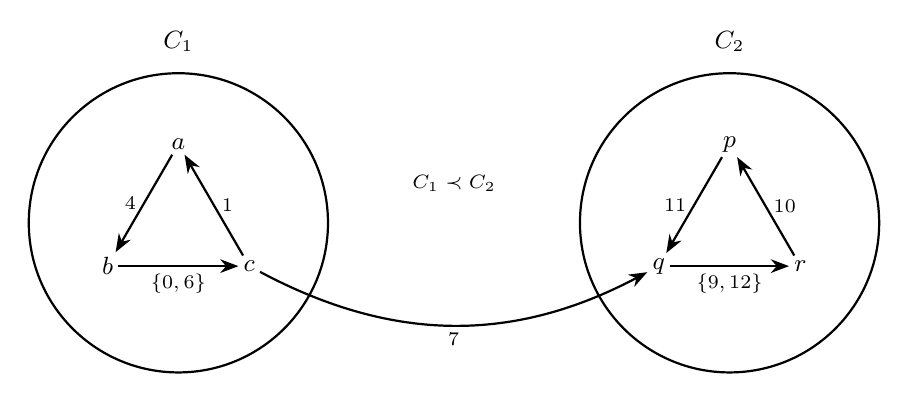
\begin{tikzpicture}[>=Stealth, thick, font=\small, every node/.style={inner sep=1.5pt}]
  % --- C_1 ---
  \draw (0,0) circle (1.9cm);
  \node at (0,2.3) {$C_1$};
  \node (a) at (0,1.0)      {$a$};
  \node (b) at (-0.9,-0.55) {$b$};
  \node (c) at (0.9,-0.55)  {$c$};
  \draw[->] (a) -- node[left=1pt,font=\scriptsize]{$4$}        (b);
  \draw[->] (b) -- node[below=1pt,font=\scriptsize]{$\{0,6\}$} (c);
  \draw[->] (c) -- node[right=1pt,font=\scriptsize]{$1$}       (a);
  % --- C_2 ---
  \draw (7,0) circle (1.9cm);
  \node at (7,2.3) {$C_2$};
  \node (p) at (7,1.0)      {$p$};
  \node (q) at (6.1,-0.55)  {$q$};
  \node (r) at (7.9,-0.55)  {$r$};
  \draw[->] (p) -- node[left=1pt,font=\scriptsize]{$11$}        (q);
  \draw[->] (q) -- node[below=1pt,font=\scriptsize]{$\{9,12\}$} (r);
  \draw[->] (r) -- node[right=1pt,font=\scriptsize]{$10$}       (p);
  % --- cross edge ---
  \draw[->] (c) to[bend right=28] node[midway,below=1pt,font=\scriptsize]{$7$} (q);
  \node[font=\scriptsize] at (3.5,0.5) {$C_1\prec C_2$};
\end{tikzpicture}
\caption{The worked example: two SCCs $C_1$ (center $h_1=a$) and $C_2$ (center $h_2=p$), each a
directed triangle, joined by the cross edge $c\to q$. The number(s) on each edge are its assigned
label(s), computed below; an edge lying on both trees, such as $(b,c)$ or $(q,r)$, carries two labels,
while the cross edge $c\to q$ carries $t_{\mathrm{cross}}=7$. Travel times $w$ are listed in the text.}
\label{fig:example}
\end{figure}

\paragraph{Component $C_1$ ($T_1=0$).} Take $h_1=a$. Inside $C_1$ the in-tree is $b\to c\to a$ (with
$\din(a)=0$, $\din(c)=3$, $\din(b)=4$) and the out-tree is $a\to b\to c$ (with $\dout(a)=0$,
$\dout(b)=2$, $\dout(c)=3$), so $D^{(1)}_{\mathrm{in}}=4$ and $D^{(1)}_{\mathrm{out}}=3$. The labels are
\[
  \begin{array}{l@{\qquad}l}
    \text{in-tree }(b,c):\ t_{\mathrm{in}}=0+4-4=0,  & \text{in-tree }(c,a):\ t_{\mathrm{in}}=0+4-3=1,\\[2pt]
    \text{out-tree }(a,b):\ t_{\mathrm{out}}=0+4+0=4, & \text{out-tree }(b,c):\ t_{\mathrm{out}}=0+4+2=6.
  \end{array}
\]
Edge $(b,c)$ lies on both trees, so it carries two labels $\{0,6\}$; every other edge carries one.

\emph{An intra-component demand $c\to b$.} Its canonical route climbs the in-tree to $a$ and descends
the out-tree, i.e.\ $c\to a\to b$, giving the schedule (edge\,@\,departure time)
\[
  (c,a)\,@\,1\ \longrightarrow\ (a,b)\,@\,4,
\]
which reaches the center $a$ at time $T_1+D^{(1)}_{\mathrm{in}}=4$ and $b$ at time
$T_1+D^{(1)}_{\mathrm{in}}+\dout(b)=6$. Each departure is at least the previous arrival, so it is a
temporal path (proved in general in \S\ref{sec:feasibility}).

\paragraph{The cross edge and the base time $T_2$.} Edge $c\to q$ receives the single label
$t_{\mathrm{cross}}(c,q)=T_1+D^{(1)}_{\mathrm{in}}+D^{(1)}_{\mathrm{out}}=0+4+3=7$, the latest time
$C_1$ ever issues. By~\eqref{eq:basetime},
\[
  T_2=\max\bigl\{\,T_1+1,\ \ T_1+D^{(1)}_{\mathrm{in}}+D^{(1)}_{\mathrm{out}}+w(c,q)\,\bigr\}
     =\max\{\,1,\ 7+2\,\}=9,
\]
so $C_2$ opens late enough to catch whatever arrives through $c\to q$.

\paragraph{Component $C_2$ ($T_2=9$).} With $h_2=p$, the in-tree $q\to r\to p$ has $\din(p)=0$,
$\din(r)=1$, $\din(q)=2$ and the out-tree $p\to q\to r$ has $\dout(p)=0$, $\dout(q)=1$, $\dout(r)=2$,
so $D^{(2)}_{\mathrm{in}}=D^{(2)}_{\mathrm{out}}=2$ and
\[
  \begin{array}{l@{\qquad}l}
    \text{in-tree }(q,r):\ t_{\mathrm{in}}=9+2-2=9,   & \text{in-tree }(r,p):\ t_{\mathrm{in}}=9+2-1=10,\\[2pt]
    \text{out-tree }(p,q):\ t_{\mathrm{out}}=9+2+0=11, & \text{out-tree }(q,r):\ t_{\mathrm{out}}=9+2+1=12.
  \end{array}
\]
Again $(q,r)$ carries two labels, $\{9,12\}$.

\emph{An inter-component demand $a\to r$.} Its canonical route descends $C_1$'s out-tree to the exit
$c$, crosses to $q$, then climbs $C_2$'s in-tree to $p$ and descends to $r$:
\[
  a\to b\to c\ \xrightarrow{\ \mathrm{cross}\ }\ q\to r\to p\to q\to r,
\]
with schedule
\[
  (a,b)\,@\,4\ \to\ (b,c)\,@\,6\ \to\ (c,q)\,@\,7\ \to\ (q,r)\,@\,9\ \to\ (r,p)\,@\,10\ \to\ (p,q)\,@\,11\ \to\ (q,r)\,@\,12,
\]
arriving at $r$ at time $13$. Every departure is at least the preceding arrival, so the route is a
temporal path. Note how the cross label $7$ and the base time $T_2=9$ dovetail: the flow leaves $C_1$
at time $7$ and reaches $q$ at $7+w(c,q)=9=T_2$, exactly when $C_2$'s schedule opens.

%====================================================================
\section{Analysis}\label{sec:feasibility}
%====================================================================

With the algorithm fully described, we prove that it is correct---the labelled backbone lets every
demand travel (\S\ref{sec:tempconn})---that each backbone edge carries at most two labels
(\S\ref{sec:twolabel}), and finally we bound its approximation ratio (\S\ref{sec:ratio}).

\subsection{The labelled backbone is temporally connected}\label{sec:tempconn}

\begin{lemma}[Intra-component temporal path]\label{lem:intra}
Let $u,v$ lie in the same component $C_i$, and suppose the flow is available at $u$ by time
$T_i+\Din-\din(u)$. Then the canonical route $u\to\cdots\to h_i\to\cdots\to v$ is a temporal path: the
flow departs each edge exactly at its label, reaches $h_i$ at time $T_i+\Din$, and reaches $v$ at time
$T_i+\Din+\dout(v)$. In particular $u$ and $v$ are temporally connected, and the segment occupies the
time window $[\,T_i,\;T_i+\Din+\Dout\,]$.
\end{lemma}

\begin{proof}
\emph{Ascent.} Along the in-tree path $u=x_0\to\cdots\to x_p=h_i$ with $e_k=(x_k,x_{k+1})\in\Tin$,
\eqref{eq:treerec} gives $\din(x_k)=w(e_k)+\din(x_{k+1})$. Departing $x_k$ at
$t_{\mathrm{in}}(e_k)=T_i+\Din-\din(x_k)$, the flow reaches $x_{k+1}$ at
\[
  \bigl(T_i+\Din-\din(x_k)\bigr)+w(e_k)=T_i+\Din-\din(x_{k+1})=t_{\mathrm{in}}(e_{k+1}),
\]
so each hop is time-respecting with no waiting, and the flow reaches $h_i$ at $T_i+\Din$ (as
$\din(h_i)=0$).

\emph{Descent.} Along the out-tree path $h_i=y_0\to\cdots\to y_q=v$ with $g_k=(y_k,y_{k+1})\in\Tout$
and $\dout(y_{k+1})=\dout(y_k)+w(g_k)$ by~\eqref{eq:treerec}, the first edge departs $h_i$ at
$t_{\mathrm{out}}(g_0)=T_i+\Din+\dout(h_i)=T_i+\Din$, exactly the arrival at $h_i$; inductively the
flow reaches $y_{k+1}$ at $T_i+\Din+\dout(y_{k+1})=t_{\mathrm{out}}(g_{k+1})$. The concatenation is a
temporal path ending at $T_i+\Din+\dout(v)\le T_i+\Din+\Dout$.
\end{proof}

\begin{lemma}[Cross edges preserve temporality]\label{lem:cross}
Let $c=(a,b)$ be a cross edge with $a\in C_i$ and $b\in C_j$ ($i<j$). Under the base
times~\eqref{eq:basetime}, the flow reaches $a$ no later than $t_{\mathrm{cross}}(c)=T_i+\Din+\Dout$,
departs $c$ at that label, and reaches $b$ by time $T_j$. Hence the cross hop together with the
hand-off into $C_j$ is time-respecting.
\end{lemma}

\begin{proof}
By the canonical route, $a$ is the exit vertex of $C_i$, reached by descending the out-tree; hence by
the descent in Lemma~\ref{lem:intra} the flow arrives at $a$ at time
\[
  T_i+\Din+\dout(a)\;\le\;T_i+\Din+\Dout=t_{\mathrm{cross}}(c),
\]
using $\dout(a)\le\Dout$. Since $t_{\mathrm{cross}}(c)$ is the only label of $c$, the flow (waiting if
necessary) departs $c$ at $t_{\mathrm{cross}}(c)$ and arrives at $b$ at $t_{\mathrm{cross}}(c)+w(c)$.
By~\eqref{eq:basetime}, $T_j\ge T_i+\Din+\Dout+w(c)=t_{\mathrm{cross}}(c)+w(c)$, so the flow reaches
$b$ by $T_j$. Finally the in-tree departure at $b$ is $T_j+D^{(j)}_{\mathrm{in}}-\din(b)\ge T_j$, so
the flow waits at $b$ and continues up $C_j$'s in-tree; the hand-off is time-respecting.
\end{proof}

\begin{figure}[H]
\centering
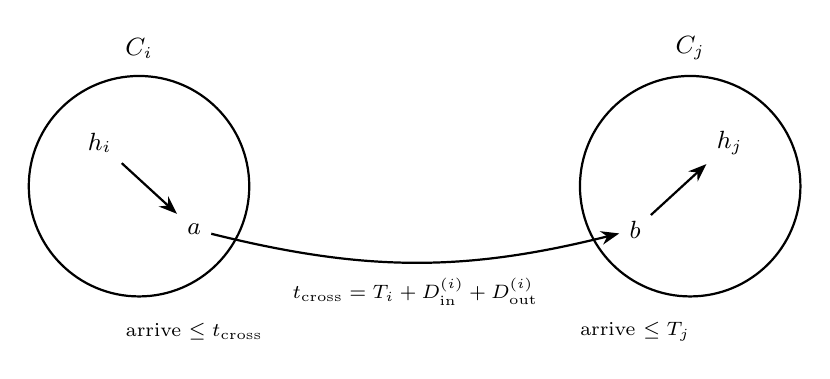
\begin{tikzpicture}[>=Stealth, thick, font=\small]
    \draw (0,0) circle (1.4cm);
    \node at (0,1.75) {$C_i$};
    \node (hi) at (-0.5,0.55) {$h_i$};
    \node (a)  at (0.7,-0.55) {$a$};
    \draw[->] (hi) -- (a);
    \draw (7,0) circle (1.4cm);
    \node at (7,1.75) {$C_j$};
    \node (b)  at (6.3,-0.55) {$b$};
    \node (hj) at (7.5,0.55) {$h_j$};
    \draw[->] (b) -- (hj);
    \draw[->] (a) to[bend right=14] node[midway,below=2pt,font=\scriptsize]
        {$t_{\mathrm{cross}}=T_i+\Din+\Dout$} (b);
    \node[font=\scriptsize] at (0.7,-1.85) {arrive $\le t_{\mathrm{cross}}$};
    \node[font=\scriptsize] at (6.3,-1.85) {arrive $\le T_j$};
\end{tikzpicture}
\caption{Cross edge $c=(a,b)$, $a\in C_i$, $b\in C_j$ (Lemma~\ref{lem:cross}). Descending $C_i$'s
out-tree, the flow reaches the exit $a$ by $t_{\mathrm{cross}}=T_i+\Din+\Dout$; it departs $c$ at
$t_{\mathrm{cross}}$ and reaches the entry $b$ of $C_j$ by $T_j\ge t_{\mathrm{cross}}+w(c)$, then waits
for $C_j$'s in-tree schedule ($\ge T_j$).}
\label{fig:cross}
\end{figure}

\begin{theorem}[The labelled backbone is temporally connected]\label{thm:temporal}
For every terminal pair $(u,v)$ joined through the backbone---within one component or across
several---the canonical route $R(u,v)$ is a temporal path. Hence $(\GSF,\lambda)$ is temporally
connected on all terminal pairs, and all backbone flows can be routed simultaneously.
\end{theorem}

\begin{proof}
Induct on the number $m$ of cross edges of $R(u,v)$. If $m=0$ then $u,v$ share a component and $R(u,v)$
is a temporal path by Lemma~\ref{lem:intra}. For the step, assume the prefix of $R(u,v)$ delivers the
flow to the entry vertex of component $C_{i_l}$ by time $T_{i_l}$ (initially this holds, since the
source is released at its in-tree label). The segment inside $C_{i_l}$ is a temporal path by
Lemma~\ref{lem:intra} (the entry arrives by $T_{i_l}$, which is at most its in-tree departure), and
the following cross edge with the hand-off into $C_{i_{l+1}}$ is time-respecting by
Lemma~\ref{lem:cross}, delivering the flow to the next entry vertex by $T_{i_{l+1}}$. Splicing
time-respecting sub-walks yields a temporal path.
\end{proof}

\subsection{At most two labels per edge}\label{sec:twolabel}

\begin{theorem}[Two labels per edge and consolidation]\label{thm:twolabels}
$\textsc{Assign-Labels}$ assigns at most two distinct labels to every backbone edge, and every
fractional flow routed on a common edge departs on those labels. Hence each backbone edge incurs at
most two round-ups in the objective~\eqref{eq:objective}.
\end{theorem}

\begin{proof}
Inside a component the in-tree and out-tree are arborescences of opposite orientation (towards,
respectively away from, the center). A directed edge $e=(x,y)$ may belong to the in-tree---carrying
ascending flow with label $t_{\mathrm{in}}(e)$---and simultaneously to the out-tree---carrying
descending flow with label $t_{\mathrm{out}}(e)$---as happens on a directed cycle $h_i\to x\to y\to h_i$,
but to no third role; a cross edge lies on neither tree and carries only $t_{\mathrm{cross}}(e)$. Hence
every edge has at most two labels. By Theorem~\ref{thm:temporal} each demand's canonical route is a
temporal path that leaves $e$ exactly on the label of the role in which it uses $e$, so all demands
using $e$ in the same role depart together; the vehicles on $e$ therefore number at most
$\lceil f_{t_1}(e)\rceil+\lceil f_{t_2}(e)\rceil$, i.e.\ at most two round-ups.
\end{proof}

\subsection{Approximation ratio}\label{sec:ratio}

For a minimization problem, an algorithm is an \emph{$r$-approximation} if its cost is at most
$r\cdot\OPT$ on every instance, where $\OPT$ is the optimum of~\eqref{eq:objective}. We write
$\ALG=\ALGSP+\ALGSF$ for the cost split by track and bound $\ALG/\OPT$. Although $\OPT$ is unknown, it
exceeds two ideal quantities.

\begin{definition}[Lower bounds]\label{def:lb}
\leavevmode
\begin{itemize}[topsep=2pt,itemsep=2pt]
  \item \textbf{Fractional-flow bound $\OPTfrac$:} the cost if fractional vehicles were allowed (no
        round-up) and all flow went on shortest paths,
        $\OPTfrac=\sum_{i=1}^{h}\dem(d_i)\cdot\len(\SP_i)$. Since every unit is forced to round up in
        reality, $\OPT\ge\OPTfrac$.
  \item \textbf{Connectivity bound $\OPTSF$:} however small a flow is, each source must reach its
        destination, so the optimal solution contains a directed path per terminal pair, i.e.\ a
        Directed Steiner Forest; with unit edge cost the minimum DSF size is a floor, $\OPT\ge\OPTSF$.
\end{itemize}
\end{definition}

\noindent Let $\rho_{\mathrm{DSF}}=O(n^{2/3})$ be the DSF approximation factor of~\cite{BBMRY13} used
in $\textsc{Build-Backbone}$ (we suppress the arbitrarily small $\epsilon$); then
$|\ESF|\le\rho_{\mathrm{DSF}}\cdot\OPTSF=O(n^{2/3})\cdot\OPTSF$.

\paragraph{Shortest-path track.} The SP track carries the integer parts $d_I$ and the leftover
fractional pieces $x=d_f-\theta$ (for demands with $d_f>2\theta$). Integer flow never wastes a
vehicle, since $\lceil\sum d_I\rceil=\sum d_I$; hence
\begin{equation}\label{eq:spint}
  \ALGSP^{\mathrm{int}}=\sum_{i=1}^{h} d_I^{(i)}\cdot\len(\SP_i)
  \;\le\;\sum_{i=1}^{h}\dem(d_i)\cdot\len(\SP_i)=\OPTfrac .
\end{equation}
A leftover piece exists only when $d_f>2\theta$, in which case $x=d_f-\theta>2\theta-\theta=\theta$; so
each such piece rounds up to $\lceil x\rceil=1$ vehicle per edge, and using $x>\theta\Rightarrow1<x/\theta$,
\begin{equation}\label{eq:spfrac}
  \ALGSP^{\mathrm{frac}}
  =\!\!\sum_{i:\,d_f>2\theta}\!\!1\cdot\len(\SP_i)
  \;<\!\!\sum_{i:\,d_f>2\theta}\!\!\frac{x_i}{\theta}\,\len(\SP_i)
  =\frac1\theta\!\!\sum_{i:\,d_f>2\theta}\!\! x_i\,\len(\SP_i)
  \;\le\;\frac1\theta\,\OPTfrac,
\end{equation}
where the last step uses $x_i\le\dem(d_i)$ and that the leftover pieces form a subset of the total
flow, so $\sum x_i\len(\SP_i)\le\sum_i\dem(d_i)\len(\SP_i)=\OPTfrac$. Adding \eqref{eq:spint}
and~\eqref{eq:spfrac},
\begin{equation}\label{eq:sp}
  \boxed{\;\ALGSP \;\le\; \Bigl(1+\tfrac1\theta\Bigr)\OPTfrac \;=\; O\!\Bigl(\tfrac1\theta\Bigr)\cdot\OPT.\;}
\end{equation}

\paragraph{Steiner-forest track.} Every demand injects at most $2\theta$ of flow into the backbone
($d_f\le2\theta$ if $d_f\le2\theta$, else exactly $\theta$). Let demand $i$ route its backbone flow
$s_i\le2\theta$ along its canonical route $R_i$. For a backbone edge $e$, let $f_{t_1}(e),f_{t_2}(e)$
be the flows departing on its (at most two) labels, and put $F_e=f_{t_1}(e)+f_{t_2}(e)$, the total
flow dispatched on $e$ across its labels. By Theorem~\ref{thm:twolabels} the vehicles on $e$ number
$\lceil f_{t_1}(e)\rceil+\lceil f_{t_2}(e)\rceil\le F_e+2$; summing over all edges,
\begin{equation}\label{eq:sfsum}
  \ALGSF \;\le\; \sum_{e\in\ESF}(F_e+2)
  \;=\;\underbrace{\sum_{e\in\ESF}F_e}_{\text{flow term}}\;+\;\underbrace{2\,|\ESF|}_{\text{infrastructure term}}.
\end{equation}
A canonical route traverses each backbone edge at most twice---at most once as an in-tree (ascent)
edge and at most once as an out-tree (descent) edge, and each cross edge at most once---so
$|R_i|\le 2|\ESF|$ (counting multiplicity). Since $\sum_{e}F_e$ totals the flow dispatched over all
edges and labels, it equals $\sum_i s_i\,|R_i|$; hence
\begin{equation}\label{eq:flowterm}
  \sum_{e\in\ESF}F_e=\sum_{i=1}^{h} s_i\,|R_i|
  \;\le\; 2\theta\sum_{i=1}^{h}|R_i|
  \;\le\; 2\theta\cdot h\cdot 2|\ESF| \;=\; 4h\theta\,|\ESF| .
\end{equation}
The infrastructure term is unavoidable: an edge carrying any positive flow dispatches a whole vehicle
per label, i.e.\ at most $2$ vehicles, giving $2|\ESF|$; this term is independent of $\theta$ and must
not be dropped. Combining \eqref{eq:sfsum}--\eqref{eq:flowterm} with $|\ESF|\le O(n^{2/3})\OPTSF$,
\begin{equation}\label{eq:sf}
  \boxed{\;\ALGSF \;\le\; (4h\theta+2)\,|\ESF|
  \;=\; O\!\bigl((h\theta+1)\,n^{2/3}\bigr)\cdot\OPTSF
  \;\le\; O\!\bigl((h\theta+1)\,n^{2/3}\bigr)\cdot\OPT.\;}
\end{equation}

\paragraph{Balancing the two tracks.} For a fixed $\theta$, write $\mathrm{TotalRatio}(\theta)$ for the
upper bound our analysis proves on $\ALG/\OPT=(\ALGSP+\ALGSF)/\OPT$. Adding \eqref{eq:sp}
and~\eqref{eq:sf},
\begin{equation}\label{eq:total}
  \frac{\ALG}{\OPT}\;\le\;\mathrm{TotalRatio}(\theta)
  \;=\; O\!\Bigl(\tfrac1\theta\Bigr)\;+\;O\!\bigl(h\theta\,n^{2/3}\bigr)\;+\;O\!\bigl(n^{2/3}\bigr).
\end{equation}
Only the first two terms depend on $\theta$; equating them,
\begin{equation}\label{eq:thetastar}
  \frac1\theta = h\theta\,n^{2/3}
  \;\Longrightarrow\; \theta^\ast=\frac{1}{\sqrt{h}\,n^{1/3}}\in(0,1).
\end{equation}
At $\theta^\ast$ each of the first two terms equals $\sqrt{h}\,n^{1/3}$, while the third is unchanged:
\begin{equation}\label{eq:final}
  \boxed{\;\mathrm{TotalRatio}(\theta^\ast)
  \;=\; O\!\bigl(\sqrt{h}\,n^{1/3}+n^{2/3}\bigr)
  \;=\; O\!\bigl(\max\{\sqrt{h}\,n^{1/3},\,n^{2/3}\}\bigr).\;}
\end{equation}

\begin{theorem}[Approximation guarantee]\label{thm:main}
Algorithm~\ref{alg:main} with threshold $\theta^\ast=1/(\sqrt{h}\,n^{1/3})$ runs in polynomial time and
returns a feasible labelling and routing whose cost is within a factor
$O\!\bigl(\sqrt{h}\,n^{1/3}+n^{2/3}\bigr)$ of the optimum of~\eqref{eq:objective}.
\end{theorem}

\begin{remark}[Two regimes]
The bound~\eqref{eq:final} splits at $h=n^{2/3}$: it is $O(\sqrt{h}\,n^{1/3})$ when $h\ge n^{2/3}$
(round-up dominated) and $O(n^{2/3})$ when $h<n^{2/3}$ (backbone dominated). When demands are plentiful
the flow-splitting is what limits the cost; when they are few the cost is governed by the Directed
Steiner Forest approximation factor $O(n^{2/3})$, which no choice of $\theta$ can remove, since the
backbone must be built to enable consolidation.
\end{remark}

\begin{remark}[On a common pitfall]
Dropping the infrastructure term $2|\ESF|$ in~\eqref{eq:sfsum}---folding it into
$O(h\theta\,n^{2/3})$---is valid only when $h\theta\ge1$. But $h\theta^\ast=\sqrt{h}/n^{1/3}<1$ whenever
$h<n^{2/3}$, so the additive term in fact dominates there; retaining it yields the honest
bound~\eqref{eq:final}, whereas omitting it would incorrectly claim $O(\sqrt{h}\,n^{1/3})$.
\end{remark}

%====================================================================
\section{Conclusion}\label{sec:conclusion}
%====================================================================

We gave a polynomial-time $O\!\bigl(\sqrt{h}\,n^{1/3}+n^{2/3}\bigr)$-approximation for MAL-C. The
algorithm sends bulky integer flow along shortest paths and consolidates fractional flow onto a
Directed Steiner Forest backbone, splitting the two at a threshold $\theta^\ast=1/(\sqrt{h}\,n^{1/3})$.
The backbone labelling makes every terminal pair temporally connected while giving each edge at most
two labels, so consolidated flows share vehicles and almost no rounding occurs. The bound is round-up
dominated when $h\ge n^{2/3}$ and backbone dominated otherwise, the latter reflecting the intrinsic
cost of the Directed Steiner Forest approximation.

\begin{thebibliography}{9}
\bibitem{BBMRY13}
P.~Berman, A.~Bhattacharyya, K.~Makarychev, S.~Raskhodnikova, and G.~Yaroslavtsev.
\newblock Approximation algorithms for spanner problems and Directed Steiner Forest.
\newblock \emph{Information and Computation}, 222:93--107, 2013.

\bibitem{CDO25}
D.~Carnevale, G.~D'Angelo, and M.~Olsen.
\newblock Approximating optimal labelings for temporal connectivity.
\newblock In \emph{AAAI}, 2025.
\end{thebibliography}

\end{document}
